% This file was created with tikzplotlib v0.10.1.
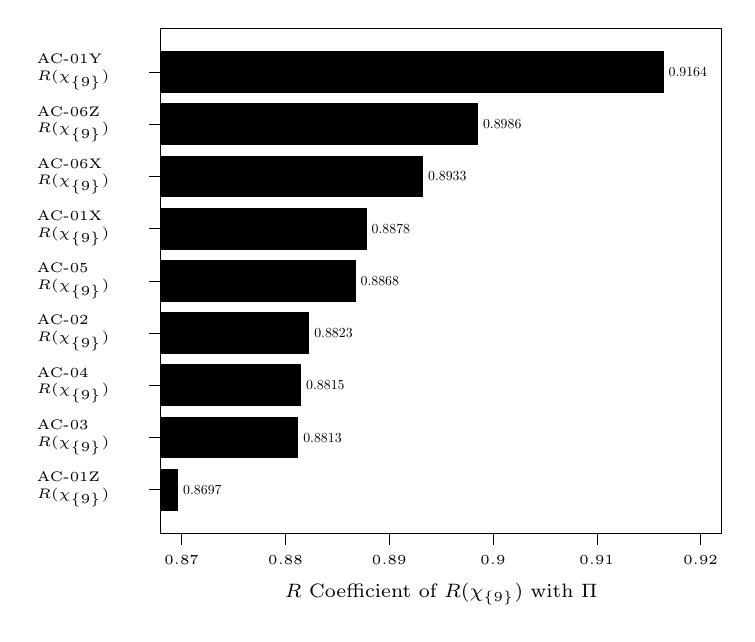
\begin{tikzpicture}

\definecolor{darkgray176}{RGB}{176,176,176}
\definecolor{sienna1279963}{RGB}{127,99,63}
\pgfplotsset{every tick label/.append style={font=\tiny}}

\begin{axis}[
tick align=outside,
tick pos=left,
x grid style={darkgray176},
xlabel={\scriptsize {$R$ Coefficient of $\mathbb{R}(\boldsymbol{\chi}_{\{ 9 \}})$ with $\boldsymbol{\Pi}$}},
xmin=0.868, xmax=0.922,
xtick style={color=black},
y grid style={darkgray176},
ymin=-0.84, ymax=8.84,
ytick style={color=black},
ytick = {0, 1, 2, 3, 4, 5, 6, 7, 8},
yticklabels= {
\parbox{13mm}{AC-01Z $\mathbb{R}(\boldsymbol{\chi}_{\{ 9 \}})  $},
\parbox{13mm}{AC-03  $\mathbb{R}(\boldsymbol{\chi}_{\{ 9 \}})  $}, 
\parbox{13mm}{AC-04  $\mathbb{R}(\boldsymbol{\chi}_{\{ 9 \}})  $}, 
\parbox{13mm}{AC-02  $\mathbb{R}(\boldsymbol{\chi}_{\{ 9 \}})  $}, 
\parbox{13mm}{AC-05  $\mathbb{R}(\boldsymbol{\chi}_{\{ 9 \}})  $}, 
\parbox{13mm}{AC-01X $\mathbb{R}(\boldsymbol{\chi}_{\{ 9 \}})  $}, 
\parbox{13mm}{AC-06X $\mathbb{R}(\boldsymbol{\chi}_{\{ 9 \}})  $}, 
\parbox{13mm}{AC-06Z $\mathbb{R}(\boldsymbol{\chi}_{\{ 9 \}})  $}, 
\parbox{13mm}{AC-01Y $\mathbb{R}(\boldsymbol{\chi}_{\{ 9 \}})  $}, 
},
height=80mm,
width=87mm,
]
\draw[draw=none,fill=black] (axis cs:0,-0.4)rectangle (axis cs:0.869683664287886,0.4);
\draw[draw=none,fill=black] (axis cs:0,0.6) rectangle (axis cs:0.881251568666528,1.4);
\draw[draw=none,fill=black] (axis cs:0,1.6) rectangle (axis cs:0.881532240479358,2.4);
\draw[draw=none,fill=black] (axis cs:0,2.6) rectangle (axis cs:0.882312767527318,3.4);
\draw[draw=none,fill=black] (axis cs:0,3.6) rectangle (axis cs:0.886772687275304,4.4);
\draw[draw=none,fill=black] (axis cs:0,4.6) rectangle (axis cs:0.887845349607805,5.4);
\draw[draw=none,fill=black] (axis cs:0,5.6) rectangle (axis cs:0.893280103396995,6.4);
\draw[draw=none,fill=black] (axis cs:0,6.6) rectangle (axis cs:0.898571596447509,7.4);
\draw[draw=none,fill=black] (axis cs:0,7.6) rectangle (axis cs:0.916447753679064,8.4);
\draw (axis cs:0.869683664287886,0) ++(0pt,0pt) node[
  scale=0.5,
  anchor=west,
  text=black,
  rotate=0.0
]{0.8697};
\draw (axis cs:0.881251568666528,1) ++(0pt,0pt) node[
  scale=0.5,
  anchor=west,
  text=black,
  rotate=0.0
]{0.8813};
\draw (axis cs:0.881532240479358,2) ++(0pt,0pt) node[
  scale=0.5,
  anchor=west,
  text=black,
  rotate=0.0
]{0.8815};
\draw (axis cs:0.882312767527318,3) ++(0pt,0pt) node[
  scale=0.5,
  anchor=west,
  text=black,
  rotate=0.0
]{0.8823};
\draw (axis cs:0.886772687275304,4) ++(0pt,0pt) node[
  scale=0.5,
  anchor=west,
  text=black,
  rotate=0.0
]{0.8868};
\draw (axis cs:0.887845349607805,5) ++(0pt,0pt) node[
  scale=0.5,
  anchor=west,
  text=black,
  rotate=0.0
]{0.8878};
\draw (axis cs:0.893280103396995,6) ++(0pt,0pt) node[
  scale=0.5,
  anchor=west,
  text=black,
  rotate=0.0
]{0.8933};
\draw (axis cs:0.898571596447509,7) ++(0pt,0pt) node[
  scale=0.5,
  anchor=west,
  text=black,
  rotate=0.0
]{0.8986};
\draw (axis cs:0.916447753679064,8) ++(0pt,0pt) node[
  scale=0.5,
  anchor=west,
  text=black,
  rotate=0.0
]{0.9164};

\end{axis}

\end{tikzpicture}
